\documentclass[1p]{elsarticle_modified}
%\bibliographystyle{elsarticle-num}

%\usepackage[colorlinks]{hyperref}
%\usepackage{abbrmath_seonhwa} %\Abb, \Ascr, \Acal ,\Abf, \Afrak
\usepackage{amsfonts}
\usepackage{amssymb}
\usepackage{amsmath}
\usepackage{amsthm}
\usepackage{scalefnt}
\usepackage{amsbsy}
\usepackage{kotex}
\usepackage{caption}
\usepackage{subfig}
\usepackage{color}
\usepackage{graphicx}
\usepackage{xcolor} %% white, black, red, green, blue, cyan, magenta, yellow
\usepackage{float}
\usepackage{setspace}
\usepackage{hyperref}

\usepackage{tikz}
\usetikzlibrary{arrows}

\usepackage{multirow}
\usepackage{array} % fixed length table
\usepackage{hhline}

%%%%%%%%%%%%%%%%%%%%%
\makeatletter
\renewcommand*\env@matrix[1][\arraystretch]{%
	\edef\arraystretch{#1}%
	\hskip -\arraycolsep
	\let\@ifnextchar\new@ifnextchar
	\array{*\c@MaxMatrixCols c}}
\makeatother %https://tex.stackexchange.com/questions/14071/how-can-i-increase-the-line-spacing-in-a-matrix
%%%%%%%%%%%%%%%

\usepackage[normalem]{ulem}

\newcommand{\msout}[1]{\ifmmode\text{\sout{\ensuremath{#1}}}\else\sout{#1}\fi}
%SOURCE: \msout is \stkout macro in https://tex.stackexchange.com/questions/20609/strikeout-in-math-mode

\newcommand{\cancel}[1]{
	\ifmmode
	{\color{red}\msout{#1}}
	\else
	{\color{red}\sout{#1}}
	\fi
}

\newcommand{\add}[1]{
	{\color{blue}\uwave{#1}}
}

\newcommand{\replace}[2]{
	\ifmmode
	{\color{red}\msout{#1}}{\color{blue}\uwave{#2}}
	\else
	{\color{red}\sout{#1}}{\color{blue}\uwave{#2}}
	\fi
}

\newcommand{\Sol}{\mathcal{S}} %segment
\newcommand{\D}{D} %diagram
\newcommand{\A}{\mathcal{A}} %arc


%%%%%%%%%%%%%%%%%%%%%%%%%%%%%5 test

\def\sl{\operatorname{\textup{SL}}(2,\Cbb)}
\def\psl{\operatorname{\textup{PSL}}(2,\Cbb)}
\def\quan{\mkern 1mu \triangleright \mkern 1mu}

\theoremstyle{definition}
\newtheorem{thm}{Theorem}[section]
\newtheorem{prop}[thm]{Proposition}
\newtheorem{lem}[thm]{Lemma}
\newtheorem{ques}[thm]{Question}
\newtheorem{cor}[thm]{Corollary}
\newtheorem{defn}[thm]{Definition}
\newtheorem{exam}[thm]{Example}
\newtheorem{rmk}[thm]{Remark}
\newtheorem{alg}[thm]{Algorithm}

\newcommand{\I}{\sqrt{-1}}
\begin{document}

%\begin{frontmatter}
%
%\title{Boundary parabolic representations of knots up to 8 crossings}
%
%%% Group authors per affiliation:
%\author{Yunhi Cho} 
%\address{Department of Mathematics, University of Seoul, Seoul, Korea}
%\ead{yhcho@uos.ac.kr}
%
%
%\author{Seonhwa Kim} %\fnref{s_kim}}
%\address{Center for Geometry and Physics, Institute for Basic Science, Pohang, 37673, Korea}
%\ead{ryeona17@ibs.re.kr}
%
%\author{Hyuk Kim}
%\address{Department of Mathematical Sciences, Seoul National University, Seoul 08826, Korea}
%\ead{hyukkim@snu.ac.kr}
%
%\author{Seokbeom Yoon}
%\address{Department of Mathematical Sciences, Seoul National University, Seoul, 08826,  Korea}
%\ead{sbyoon15@snu.ac.kr}
%
%\begin{abstract}
%We find all boundary parabolic representation of knots up to 8 crossings.
%
%\end{abstract}
%\begin{keyword}
%    \MSC[2010] 57M25 
%\end{keyword}
%
%\end{frontmatter}

%\linenumbers
%\tableofcontents
%
\newcommand\colored[1]{\textcolor{white}{\rule[-0.35ex]{0.8em}{1.4ex}}\kern-0.8em\color{red} #1}%
%\newcommand\colored[1]{\textcolor{white}{ #1}\kern-2.17ex	\textcolor{white}{ #1}\kern-1.81ex	\textcolor{white}{ #1}\kern-2.15ex\color{red}#1	}

{\Large $\underline{12a_{0536}~(K12a_{0536})}$}

\setlength{\tabcolsep}{10pt}
\renewcommand{\arraystretch}{1.6}
\vspace{1cm}\begin{tabular}{m{100pt}>{\centering\arraybackslash}m{274pt}}
\multirow{5}{120pt}{
	\centering
	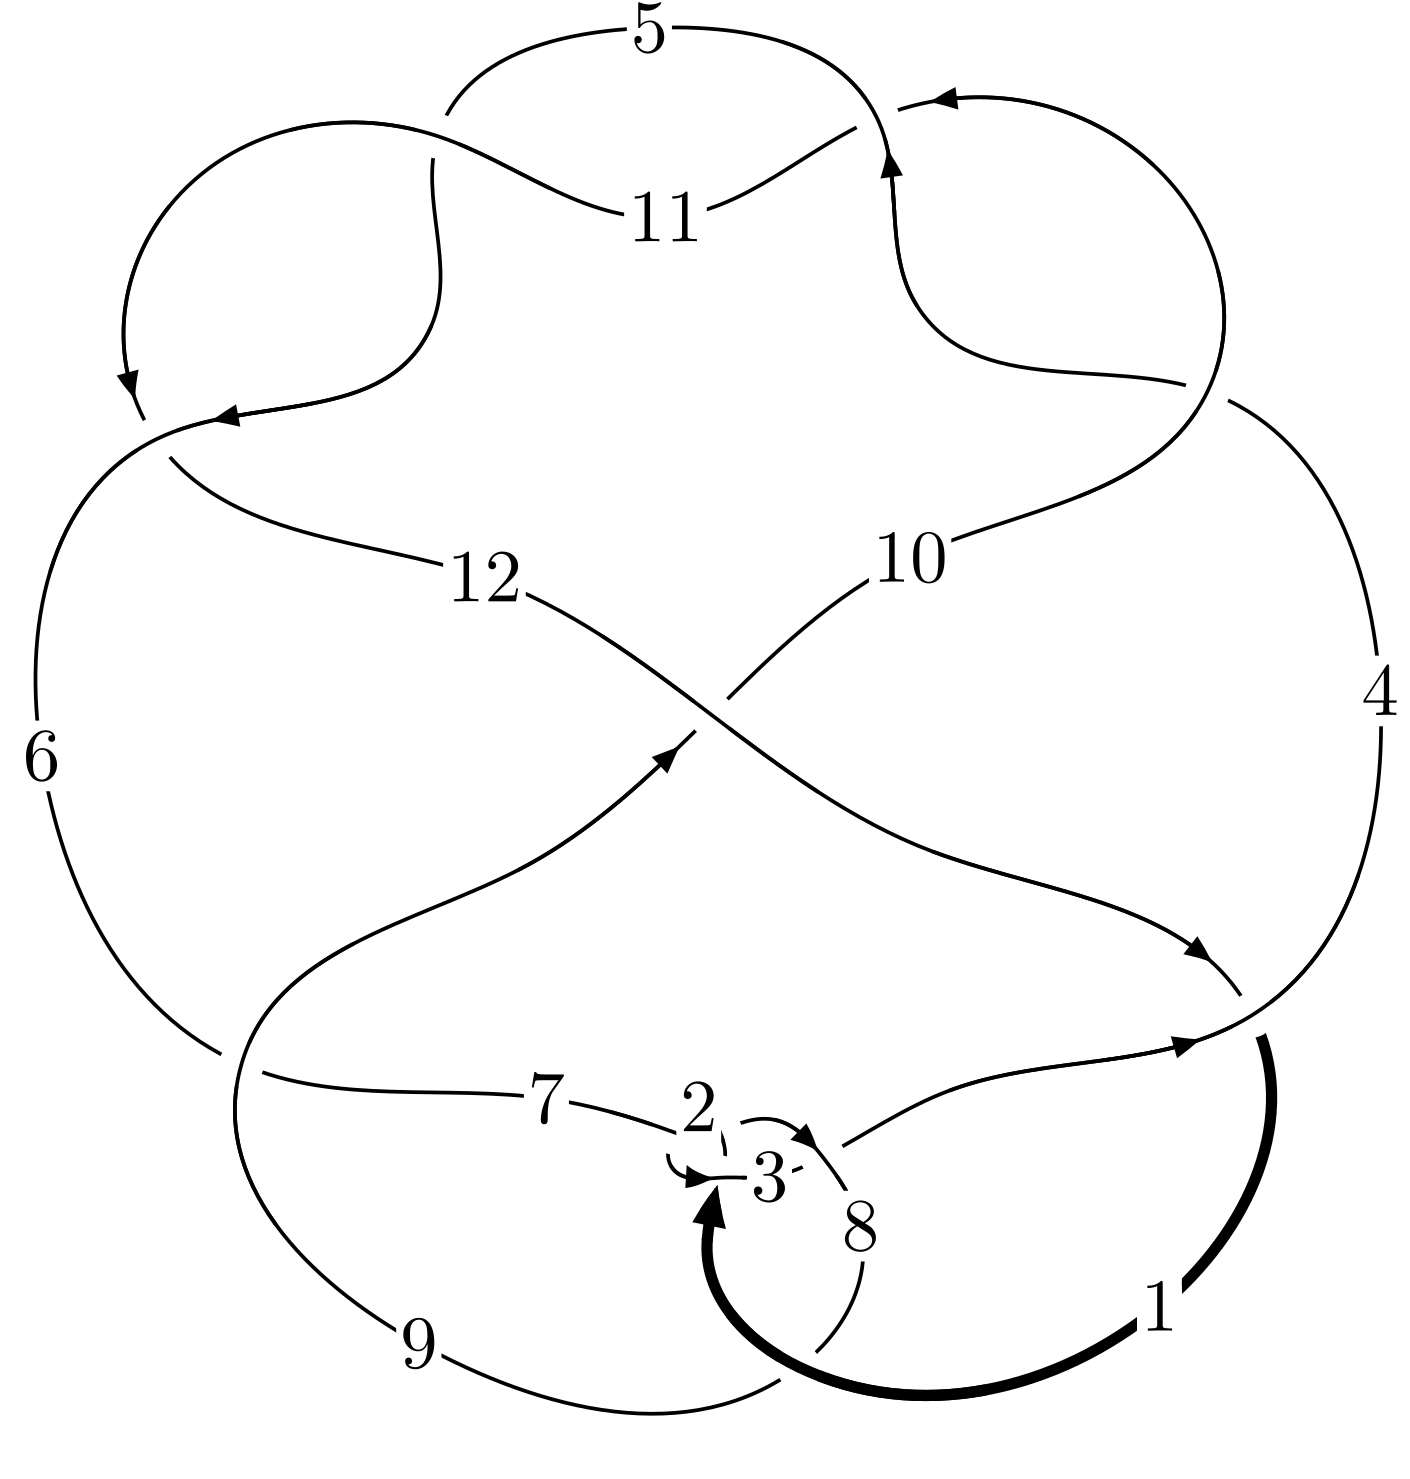
\includegraphics[width=112pt]{../../../GIT/diagram.site/Diagrams/png/1337_12a_0536.png}\\
\ \ \ A knot diagram\footnotemark}&
\allowdisplaybreaks
\textbf{Linearized knot diagam} \\
\cline{2-2}
 &
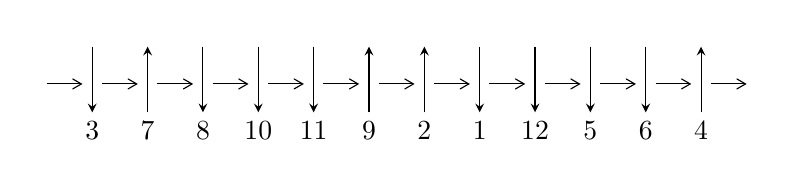
\begin{tikzpicture}[x=20pt, y=17pt]
	% nodes
	\node (C0) at (0, 0) {};
	\node (C1) at (1, 0) {};
	\node (C1U) at (1, +1) {};
	\node (C1D) at (1, -1) {3};

	\node (C2) at (2, 0) {};
	\node (C2U) at (2, +1) {};
	\node (C2D) at (2, -1) {7};

	\node (C3) at (3, 0) {};
	\node (C3U) at (3, +1) {};
	\node (C3D) at (3, -1) {8};

	\node (C4) at (4, 0) {};
	\node (C4U) at (4, +1) {};
	\node (C4D) at (4, -1) {10};

	\node (C5) at (5, 0) {};
	\node (C5U) at (5, +1) {};
	\node (C5D) at (5, -1) {11};

	\node (C6) at (6, 0) {};
	\node (C6U) at (6, +1) {};
	\node (C6D) at (6, -1) {9};

	\node (C7) at (7, 0) {};
	\node (C7U) at (7, +1) {};
	\node (C7D) at (7, -1) {2};

	\node (C8) at (8, 0) {};
	\node (C8U) at (8, +1) {};
	\node (C8D) at (8, -1) {1};

	\node (C9) at (9, 0) {};
	\node (C9U) at (9, +1) {};
	\node (C9D) at (9, -1) {12};

	\node (C10) at (10, 0) {};
	\node (C10U) at (10, +1) {};
	\node (C10D) at (10, -1) {5};

	\node (C11) at (11, 0) {};
	\node (C11U) at (11, +1) {};
	\node (C11D) at (11, -1) {6};

	\node (C12) at (12, 0) {};
	\node (C12U) at (12, +1) {};
	\node (C12D) at (12, -1) {4};
	\node (C13) at (13, 0) {};

	% arrows
	\draw[->,>={angle 60}]
	(C0) edge (C1) (C1) edge (C2) (C2) edge (C3) (C3) edge (C4) (C4) edge (C5) (C5) edge (C6) (C6) edge (C7) (C7) edge (C8) (C8) edge (C9) (C9) edge (C10) (C10) edge (C11) (C11) edge (C12) (C12) edge (C13) ;	\draw[->,>=stealth]
	(C1U) edge (C1D) (C2D) edge (C2U) (C3U) edge (C3D) (C4U) edge (C4D) (C5U) edge (C5D) (C6D) edge (C6U) (C7D) edge (C7U) (C8U) edge (C8D) (C9U) edge (C9D) (C10U) edge (C10D) (C11U) edge (C11D) (C12D) edge (C12U) ;
	\end{tikzpicture} \\
\hhline{~~} \\& 
\textbf{Solving Sequence} \\ \cline{2-2} 
 &
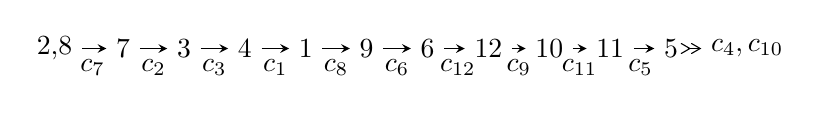
\begin{tikzpicture}[x=22pt, y=7pt]
	% node
	\node (A0) at (-1/8, 0) {2,8};
	\node (A1) at (1, 0) {7};
	\node (A2) at (2, 0) {3};
	\node (A3) at (3, 0) {4};
	\node (A4) at (4, 0) {1};
	\node (A5) at (5, 0) {9};
	\node (A6) at (6, 0) {6};
	\node (A7) at (7, 0) {12};
	\node (A8) at (8, 0) {10};
	\node (A9) at (9, 0) {11};
	\node (A10) at (10, 0) {5};
	\node (C1) at (1/2, -1) {$c_{7}$};
	\node (C2) at (3/2, -1) {$c_{2}$};
	\node (C3) at (5/2, -1) {$c_{3}$};
	\node (C4) at (7/2, -1) {$c_{1}$};
	\node (C5) at (9/2, -1) {$c_{8}$};
	\node (C6) at (11/2, -1) {$c_{6}$};
	\node (C7) at (13/2, -1) {$c_{12}$};
	\node (C8) at (15/2, -1) {$c_{9}$};
	\node (C9) at (17/2, -1) {$c_{11}$};
	\node (C10) at (19/2, -1) {$c_{5}$};
	\node (A11) at (45/4, 0) {$c_{4},c_{10}$};

	% edge
	\draw[->,>=stealth]	
	(A0) edge (A1) (A1) edge (A2) (A2) edge (A3) (A3) edge (A4) (A4) edge (A5) (A5) edge (A6) (A6) edge (A7) (A7) edge (A8) (A8) edge (A9) (A9) edge (A10) ;
	\draw[->>,>={angle 60}]	
	(A10) edge (A11);
\end{tikzpicture} \\ 

\end{tabular} \\

\footnotetext{
The image of knot diagram is generated by the software ``\textbf{Draw programme}" developed by Andrew Bartholomew(\url{http://www.layer8.co.uk/maths/draw/index.htm\#Running-draw}), where we modified some parts for our purpose(\url{https://github.com/CATsTAILs/LinksPainter}).
}\phantom \\ \newline 
\centering \textbf{Ideals for irreducible components\footnotemark of $X_{\text{par}}$} 
 
\begin{align*}
I^u_{1}&=\langle 
u^{68}+u^{67}+\cdots-2 u-1\rangle \\
\\
\end{align*}
\raggedright * 1 irreducible components of $\dim_{\mathbb{C}}=0$, with total 68 representations.\\
\footnotetext{All coefficients of polynomials are rational numbers. But the coefficients are sometimes approximated in decimal forms when there is not enough margin.}
\newpage
\renewcommand{\arraystretch}{1}
\centering \section*{I. $I^u_{1}= \langle u^{68}+u^{67}+\cdots-2 u-1 \rangle$}
\flushleft \textbf{(i) Arc colorings}\\
\begin{tabular}{m{7pt} m{180pt} m{7pt} m{180pt} }
\flushright $a_{2}=$&$\begin{pmatrix}0\\u\end{pmatrix}$ \\
\flushright $a_{8}=$&$\begin{pmatrix}1\\0\end{pmatrix}$ \\
\flushright $a_{7}=$&$\begin{pmatrix}1\\u^2\end{pmatrix}$ \\
\flushright $a_{3}=$&$\begin{pmatrix}u\\u^3+u\end{pmatrix}$ \\
\flushright $a_{4}=$&$\begin{pmatrix}- u^3\\u^3+u\end{pmatrix}$ \\
\flushright $a_{1}=$&$\begin{pmatrix}u^3\\u^5+u^3+u\end{pmatrix}$ \\
\flushright $a_{9}=$&$\begin{pmatrix}u^8+u^6+u^4+1\\u^{10}+2 u^8+3 u^6+2 u^4+u^2\end{pmatrix}$ \\
\flushright $a_{6}=$&$\begin{pmatrix}u^{16}+3 u^{14}+5 u^{12}+4 u^{10}+3 u^8+2 u^6+2 u^4+1\\u^{18}+4 u^{16}+9 u^{14}+12 u^{12}+11 u^{10}+6 u^8+2 u^6+u^2\end{pmatrix}$ \\
\flushright $a_{12}=$&$\begin{pmatrix}- u^{11}-2 u^9-2 u^7+u^3\\u^{11}+3 u^9+4 u^7+3 u^5+u^3+u\end{pmatrix}$ \\
\flushright $a_{10}=$&$\begin{pmatrix}- u^{32}-7 u^{30}+\cdots+2 u^4+1\\u^{32}+8 u^{30}+\cdots+4 u^4+2 u^2\end{pmatrix}$ \\
\flushright $a_{11}=$&$\begin{pmatrix}u^{45}+10 u^{43}+\cdots+2 u^3+u\\u^{47}+11 u^{45}+\cdots+2 u^3+u\end{pmatrix}$ \\
\flushright $a_{5}=$&$\begin{pmatrix}u^{61}+14 u^{59}+\cdots-2 u^3- u\\- u^{61}-15 u^{59}+\cdots- u^3+u\end{pmatrix}$\\&\end{tabular}
\flushleft \textbf{(ii) Obstruction class $= -1$}\\~\\
\flushleft \textbf{(iii) Cusp Shapes $= 4 u^{66}+4 u^{65}+\cdots-4 u-10$}\\~\\
\newpage\renewcommand{\arraystretch}{1}
\flushleft \textbf{(iv) u-Polynomials at the component}\newline \\
\begin{tabular}{m{50pt}|m{274pt}}
Crossings & \hspace{64pt}u-Polynomials at each crossing \\
\hline $$\begin{aligned}c_{1}\end{aligned}$$&$\begin{aligned}
&u^{68}+33 u^{67}+\cdots-2 u+1
\end{aligned}$\\
\hline $$\begin{aligned}c_{2},c_{7}\end{aligned}$$&$\begin{aligned}
&u^{68}+u^{67}+\cdots-2 u-1
\end{aligned}$\\
\hline $$\begin{aligned}c_{3}\end{aligned}$$&$\begin{aligned}
&u^{68}- u^{67}+\cdots-356 u-185
\end{aligned}$\\
\hline $$\begin{aligned}c_{4},c_{5},c_{10}\\c_{11}\end{aligned}$$&$\begin{aligned}
&u^{68}- u^{67}+\cdots-2 u-1
\end{aligned}$\\
\hline $$\begin{aligned}c_{6},c_{12}\end{aligned}$$&$\begin{aligned}
&u^{68}+5 u^{67}+\cdots+102 u+5
\end{aligned}$\\
\hline $$\begin{aligned}c_{8}\end{aligned}$$&$\begin{aligned}
&u^{68}+5 u^{67}+\cdots-4 u-3
\end{aligned}$\\
\hline $$\begin{aligned}c_{9}\end{aligned}$$&$\begin{aligned}
&u^{68}-21 u^{67}+\cdots+133900 u-11327
\end{aligned}$\\
\hline
\end{tabular}\\~\\
\newpage\renewcommand{\arraystretch}{1}
\flushleft \textbf{(v) Riley Polynomials at the component}\newline \\
\begin{tabular}{m{50pt}|m{274pt}}
Crossings & \hspace{64pt}Riley Polynomials at each crossing \\
\hline $$\begin{aligned}c_{1}\end{aligned}$$&$\begin{aligned}
&y^{68}+5 y^{67}+\cdots-22 y+1
\end{aligned}$\\
\hline $$\begin{aligned}c_{2},c_{7}\end{aligned}$$&$\begin{aligned}
&y^{68}+33 y^{67}+\cdots-2 y+1
\end{aligned}$\\
\hline $$\begin{aligned}c_{3}\end{aligned}$$&$\begin{aligned}
&y^{68}-23 y^{67}+\cdots-913726 y+34225
\end{aligned}$\\
\hline $$\begin{aligned}c_{4},c_{5},c_{10}\\c_{11}\end{aligned}$$&$\begin{aligned}
&y^{68}-79 y^{67}+\cdots-2 y+1
\end{aligned}$\\
\hline $$\begin{aligned}c_{6},c_{12}\end{aligned}$$&$\begin{aligned}
&y^{68}+57 y^{67}+\cdots-4634 y+25
\end{aligned}$\\
\hline $$\begin{aligned}c_{8}\end{aligned}$$&$\begin{aligned}
&y^{68}-3 y^{67}+\cdots-22 y+9
\end{aligned}$\\
\hline $$\begin{aligned}c_{9}\end{aligned}$$&$\begin{aligned}
&y^{68}-31 y^{67}+\cdots-1781733302 y+128300929
\end{aligned}$\\
\hline
\end{tabular}\\~\\
\newpage\flushleft \textbf{(vi) Complex Volumes and Cusp Shapes}
$$\begin{array}{c|c|c}  
\text{Solutions to }I^u_{1}& \I (\text{vol} + \sqrt{-1}CS) & \text{Cusp shape}\\
 \hline 
\begin{aligned}
u &= \phantom{-}0.569465 + 0.821421 I\end{aligned}
 & -9.88852 - 2.65108 I & -8.60098 + 0. I\phantom{ +0.000000I} \\ \hline\begin{aligned}
u &= \phantom{-}0.569465 - 0.821421 I\end{aligned}
 & -9.88852 + 2.65108 I & -8.60098 + 0. I\phantom{ +0.000000I} \\ \hline\begin{aligned}
u &= \phantom{-}0.196680 + 1.006370 I\end{aligned}
 & -8.93532 - 2.08822 I & -11.98824 + 2.12583 I \\ \hline\begin{aligned}
u &= \phantom{-}0.196680 - 1.006370 I\end{aligned}
 & -8.93532 + 2.08822 I & -11.98824 - 2.12583 I \\ \hline\begin{aligned}
u &= -0.516300 + 0.806700 I\end{aligned}
 & -1.89157 + 0.76594 I & -7.09900 - 1.49960 I \\ \hline\begin{aligned}
u &= -0.516300 - 0.806700 I\end{aligned}
 & -1.89157 - 0.76594 I & -7.09900 + 1.49960 I \\ \hline\begin{aligned}
u &= \phantom{-}0.621616 + 0.711188 I\end{aligned}
 & -9.54510 + 7.33161 I & -7.70041 - 6.15232 I \\ \hline\begin{aligned}
u &= \phantom{-}0.621616 - 0.711188 I\end{aligned}
 & -9.54510 - 7.33161 I & -7.70041 + 6.15232 I \\ \hline\begin{aligned}
u &= -0.271595 + 0.903915 I\end{aligned}
 & -1.66897 + 0.69901 I & -9.13293 - 3.92889 I \\ \hline\begin{aligned}
u &= -0.271595 - 0.903915 I\end{aligned}
 & -1.66897 - 0.69901 I & -9.13293 + 3.92889 I \\ \hline\begin{aligned}
u &= \phantom{-}0.448518 + 0.958561 I\end{aligned}
 & -0.42510 + 2.03856 I & \phantom{-0.000000 } 0 \\ \hline\begin{aligned}
u &= \phantom{-}0.448518 - 0.958561 I\end{aligned}
 & -0.42510 - 2.03856 I & \phantom{-0.000000 } 0 \\ \hline\begin{aligned}
u &= -0.597092 + 0.698260 I\end{aligned}
 & -1.52058 - 5.23538 I & -5.66765 + 8.09699 I \\ \hline\begin{aligned}
u &= -0.597092 - 0.698260 I\end{aligned}
 & -1.52058 + 5.23538 I & -5.66765 - 8.09699 I \\ \hline\begin{aligned}
u &= \phantom{-}0.543552 + 0.674693 I\end{aligned}
 & \phantom{-}0.33852 + 1.96494 I & -1.18152 - 3.58402 I \\ \hline\begin{aligned}
u &= \phantom{-}0.543552 - 0.674693 I\end{aligned}
 & \phantom{-}0.33852 - 1.96494 I & -1.18152 + 3.58402 I \\ \hline\begin{aligned}
u &= -0.542516 + 1.005270 I\end{aligned}
 & -5.43066 - 2.42556 I & \phantom{-0.000000 } 0 \\ \hline\begin{aligned}
u &= -0.542516 - 1.005270 I\end{aligned}
 & -5.43066 + 2.42556 I & \phantom{-0.000000 } 0 \\ \hline\begin{aligned}
u &= -0.444504 + 1.066540 I\end{aligned}
 & -3.39119 - 3.46853 I & \phantom{-0.000000 } 0 \\ \hline\begin{aligned}
u &= -0.444504 - 1.066540 I\end{aligned}
 & -3.39119 + 3.46853 I & \phantom{-0.000000 } 0 \\ \hline\begin{aligned}
u &= -0.779022 + 0.286596 I\end{aligned}
 & -11.6248 + 9.1994 I & -8.83810 - 4.94920 I \\ \hline\begin{aligned}
u &= -0.779022 - 0.286596 I\end{aligned}
 & -11.6248 - 9.1994 I & -8.83810 + 4.94920 I \\ \hline\begin{aligned}
u &= \phantom{-}0.533000 + 1.047100 I\end{aligned}
 & \phantom{-}0.59068 + 3.80897 I & \phantom{-0.000000 } 0 \\ \hline\begin{aligned}
u &= \phantom{-}0.533000 - 1.047100 I\end{aligned}
 & \phantom{-}0.59068 - 3.80897 I & \phantom{-0.000000 } 0 \\ \hline\begin{aligned}
u &= -0.628186 + 0.533564 I\end{aligned}
 & -4.04887 - 2.18452 I & -3.17290 + 3.27346 I \\ \hline\begin{aligned}
u &= -0.628186 - 0.533564 I\end{aligned}
 & -4.04887 + 2.18452 I & -3.17290 - 3.27346 I \\ \hline\begin{aligned}
u &= -0.285766 + 1.144430 I\end{aligned}
 & -5.69626 + 0.32025 I & \phantom{-0.000000 } 0 \\ \hline\begin{aligned}
u &= -0.285766 - 1.144430 I\end{aligned}
 & -5.69626 - 0.32025 I & \phantom{-0.000000 } 0 \\ \hline\begin{aligned}
u &= \phantom{-}0.764887 + 0.286070 I\end{aligned}
 & -3.46891 - 6.94592 I & -6.88820 + 6.61216 I \\ \hline\begin{aligned}
u &= \phantom{-}0.764887 - 0.286070 I\end{aligned}
 & -3.46891 + 6.94592 I & -6.88820 - 6.61216 I\\
 \hline 
 \end{array}$$\newpage$$\begin{array}{c|c|c}  
\text{Solutions to }I^u_{1}& \I (\text{vol} + \sqrt{-1}CS) & \text{Cusp shape}\\
 \hline 
\begin{aligned}
u &= \phantom{-}0.272050 + 1.154900 I\end{aligned}
 & -7.87704 - 3.87380 I & \phantom{-0.000000 } 0 \\ \hline\begin{aligned}
u &= \phantom{-}0.272050 - 1.154900 I\end{aligned}
 & -7.87704 + 3.87380 I & \phantom{-0.000000 } 0 \\ \hline\begin{aligned}
u &= \phantom{-}0.434060 + 1.110570 I\end{aligned}
 & -11.36200 + 3.77797 I & \phantom{-0.000000 } 0 \\ \hline\begin{aligned}
u &= \phantom{-}0.434060 - 1.110570 I\end{aligned}
 & -11.36200 - 3.77797 I & \phantom{-0.000000 } 0 \\ \hline\begin{aligned}
u &= \phantom{-}0.303760 + 1.153260 I\end{aligned}
 & -8.24956 + 3.01264 I & \phantom{-0.000000 } 0 \\ \hline\begin{aligned}
u &= \phantom{-}0.303760 - 1.153260 I\end{aligned}
 & -8.24956 - 3.01264 I & \phantom{-0.000000 } 0 \\ \hline\begin{aligned}
u &= -0.266265 + 1.165210 I\end{aligned}
 & -16.1206 + 6.0842 I & \phantom{-0.000000 } 0 \\ \hline\begin{aligned}
u &= -0.266265 - 1.165210 I\end{aligned}
 & -16.1206 - 6.0842 I & \phantom{-0.000000 } 0 \\ \hline\begin{aligned}
u &= -0.544409 + 1.070510 I\end{aligned}
 & \phantom{-}0.14008 - 7.02765 I & \phantom{-0.000000 } 0 \\ \hline\begin{aligned}
u &= -0.544409 - 1.070510 I\end{aligned}
 & \phantom{-}0.14008 + 7.02765 I & \phantom{-0.000000 } 0 \\ \hline\begin{aligned}
u &= \phantom{-}0.694347 + 0.389402 I\end{aligned}
 & -4.69547 - 4.07584 I & -4.42256 + 3.79856 I \\ \hline\begin{aligned}
u &= \phantom{-}0.694347 - 0.389402 I\end{aligned}
 & -4.69547 + 4.07584 I & -4.42256 - 3.79856 I \\ \hline\begin{aligned}
u &= -0.743742 + 0.279293 I\end{aligned}
 & -1.43487 + 3.37716 I & -3.04234 - 2.33518 I \\ \hline\begin{aligned}
u &= -0.743742 - 0.279293 I\end{aligned}
 & -1.43487 - 3.37716 I & -3.04234 + 2.33518 I \\ \hline\begin{aligned}
u &= -0.310586 + 1.165680 I\end{aligned}
 & -16.6556 - 4.9601 I & \phantom{-0.000000 } 0 \\ \hline\begin{aligned}
u &= -0.310586 - 1.165680 I\end{aligned}
 & -16.6556 + 4.9601 I & \phantom{-0.000000 } 0 \\ \hline\begin{aligned}
u &= -0.755158 + 0.228194 I\end{aligned}
 & -12.47070 - 1.60811 I & -10.06141 + 0.47911 I \\ \hline\begin{aligned}
u &= -0.755158 - 0.228194 I\end{aligned}
 & -12.47070 + 1.60811 I & -10.06141 - 0.47911 I \\ \hline\begin{aligned}
u &= \phantom{-}0.739760 + 0.247030 I\end{aligned}
 & -4.08581 - 0.20619 I & -8.44067 - 1.58802 I \\ \hline\begin{aligned}
u &= \phantom{-}0.739760 - 0.247030 I\end{aligned}
 & -4.08581 + 0.20619 I & -8.44067 + 1.58802 I \\ \hline\begin{aligned}
u &= \phantom{-}0.557735 + 1.086370 I\end{aligned}
 & -6.72622 + 8.89575 I & \phantom{-0.000000 } 0 \\ \hline\begin{aligned}
u &= \phantom{-}0.557735 - 1.086370 I\end{aligned}
 & -6.72622 - 8.89575 I & \phantom{-0.000000 } 0 \\ \hline\begin{aligned}
u &= \phantom{-}0.611409 + 0.464153 I\end{aligned}
 & \phantom{-}2.29790 + 0.72696 I & \phantom{-}1.42198 - 4.03788 I \\ \hline\begin{aligned}
u &= \phantom{-}0.611409 - 0.464153 I\end{aligned}
 & \phantom{-}2.29790 - 0.72696 I & \phantom{-}1.42198 + 4.03788 I \\ \hline\begin{aligned}
u &= -0.647080 + 0.410370 I\end{aligned}
 & \phantom{-}2.05724 + 2.36478 I & -0.10664 - 5.60599 I \\ \hline\begin{aligned}
u &= -0.647080 - 0.410370 I\end{aligned}
 & \phantom{-}2.05724 - 2.36478 I & -0.10664 + 5.60599 I \\ \hline\begin{aligned}
u &= \phantom{-}0.536182 + 1.140680 I\end{aligned}
 & -6.67249 + 5.01105 I & \phantom{-0.000000 } 0 \\ \hline\begin{aligned}
u &= \phantom{-}0.536182 - 1.140680 I\end{aligned}
 & -6.67249 - 5.01105 I & \phantom{-0.000000 } 0 \\ \hline\begin{aligned}
u &= -0.547074 + 1.135730 I\end{aligned}
 & -3.92615 - 8.25146 I & \phantom{-0.000000 } 0 \\ \hline\begin{aligned}
u &= -0.547074 - 1.135730 I\end{aligned}
 & -3.92615 + 8.25146 I & \phantom{-0.000000 } 0\\
 \hline 
 \end{array}$$\newpage$$\begin{array}{c|c|c}  
\text{Solutions to }I^u_{1}& \I (\text{vol} + \sqrt{-1}CS) & \text{Cusp shape}\\
 \hline 
\begin{aligned}
u &= -0.532240 + 1.149520 I\end{aligned}
 & -15.1491 - 3.2090 I & \phantom{-0.000000 } 0 \\ \hline\begin{aligned}
u &= -0.532240 - 1.149520 I\end{aligned}
 & -15.1491 + 3.2090 I & \phantom{-0.000000 } 0 \\ \hline\begin{aligned}
u &= \phantom{-}0.554156 + 1.140460 I\end{aligned}
 & -5.97071 + 11.90170 I & \phantom{-0.000000 } 0 \\ \hline\begin{aligned}
u &= \phantom{-}0.554156 - 1.140460 I\end{aligned}
 & -5.97071 - 11.90170 I & \phantom{-0.000000 } 0 \\ \hline\begin{aligned}
u &= -0.558002 + 1.144930 I\end{aligned}
 & -14.1477 - 14.2056 I & \phantom{-0.000000 } 0 \\ \hline\begin{aligned}
u &= -0.558002 - 1.144930 I\end{aligned}
 & -14.1477 + 14.2056 I & \phantom{-0.000000 } 0 \\ \hline\begin{aligned}
u &= \phantom{-}0.596102\phantom{ +0.000000I}\end{aligned}
 & -8.41516\phantom{ +0.000000I} & -10.1960\phantom{ +0.000000I} \\ \hline\begin{aligned}
u &= -0.419381\phantom{ +0.000000I}\end{aligned}
 & -0.927902\phantom{ +0.000000I} & -10.4430\phantom{ +0.000000I}\\
 \hline 
 \end{array}$$\newpage
\newpage\renewcommand{\arraystretch}{1}
\centering \section*{ II. u-Polynomials}
\begin{tabular}{m{50pt}|m{274pt}}
Crossings & \hspace{64pt}u-Polynomials at each crossing \\
\hline $$\begin{aligned}c_{1}\end{aligned}$$&$\begin{aligned}
&u^{68}+33 u^{67}+\cdots-2 u+1
\end{aligned}$\\
\hline $$\begin{aligned}c_{2},c_{7}\end{aligned}$$&$\begin{aligned}
&u^{68}+u^{67}+\cdots-2 u-1
\end{aligned}$\\
\hline $$\begin{aligned}c_{3}\end{aligned}$$&$\begin{aligned}
&u^{68}- u^{67}+\cdots-356 u-185
\end{aligned}$\\
\hline $$\begin{aligned}c_{4},c_{5},c_{10}\\c_{11}\end{aligned}$$&$\begin{aligned}
&u^{68}- u^{67}+\cdots-2 u-1
\end{aligned}$\\
\hline $$\begin{aligned}c_{6},c_{12}\end{aligned}$$&$\begin{aligned}
&u^{68}+5 u^{67}+\cdots+102 u+5
\end{aligned}$\\
\hline $$\begin{aligned}c_{8}\end{aligned}$$&$\begin{aligned}
&u^{68}+5 u^{67}+\cdots-4 u-3
\end{aligned}$\\
\hline $$\begin{aligned}c_{9}\end{aligned}$$&$\begin{aligned}
&u^{68}-21 u^{67}+\cdots+133900 u-11327
\end{aligned}$\\
\hline
\end{tabular}\newpage\renewcommand{\arraystretch}{1}
\centering \section*{ III. Riley Polynomials}
\begin{tabular}{m{50pt}|m{274pt}}
Crossings & \hspace{64pt}Riley Polynomials at each crossing \\
\hline $$\begin{aligned}c_{1}\end{aligned}$$&$\begin{aligned}
&y^{68}+5 y^{67}+\cdots-22 y+1
\end{aligned}$\\
\hline $$\begin{aligned}c_{2},c_{7}\end{aligned}$$&$\begin{aligned}
&y^{68}+33 y^{67}+\cdots-2 y+1
\end{aligned}$\\
\hline $$\begin{aligned}c_{3}\end{aligned}$$&$\begin{aligned}
&y^{68}-23 y^{67}+\cdots-913726 y+34225
\end{aligned}$\\
\hline $$\begin{aligned}c_{4},c_{5},c_{10}\\c_{11}\end{aligned}$$&$\begin{aligned}
&y^{68}-79 y^{67}+\cdots-2 y+1
\end{aligned}$\\
\hline $$\begin{aligned}c_{6},c_{12}\end{aligned}$$&$\begin{aligned}
&y^{68}+57 y^{67}+\cdots-4634 y+25
\end{aligned}$\\
\hline $$\begin{aligned}c_{8}\end{aligned}$$&$\begin{aligned}
&y^{68}-3 y^{67}+\cdots-22 y+9
\end{aligned}$\\
\hline $$\begin{aligned}c_{9}\end{aligned}$$&$\begin{aligned}
&y^{68}-31 y^{67}+\cdots-1781733302 y+128300929
\end{aligned}$\\
\hline
\end{tabular}
\vskip 2pc
\end{document}